% fig_halow_udp_analysis.tex — Rendimiento UDP y pérdida por BW HaLow
% Datos: thesis_symmetric_package (Feb 2025, Laboratorio UNAL)
\begin{figure}[htbp]
\centering

% --- Subfigura (a): Caudal UDP recibido ---
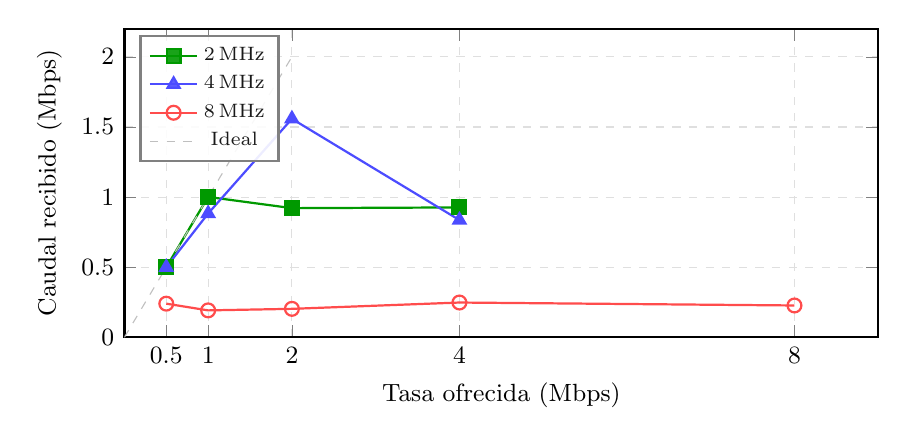
\begin{tikzpicture}
\begin{axis}[
    width=0.92\textwidth,
    height=5.5cm,
    xlabel={Tasa ofrecida (Mbps)},
    ylabel={Caudal recibido (Mbps)},
    xmin=0, xmax=9,
    ymin=0, ymax=2.2,
    xtick={0.5,1,2,4,8},
    grid=major,
    grid style={gray!25, dashed},
    tick label style={font=\small},
    label style={font=\small},
    legend style={at={(0.02,0.98)}, anchor=north west, font=\scriptsize,
                  draw=black!50, fill=white, fill opacity=0.9},
    mark size=2.5pt,
    thick,
]

% 2 MHz
\addplot[color=green!60!black, mark=square*, thick] coordinates {
    (0.5, 0.500) (1, 1.001) (2, 0.921) (4, 0.926)
};

% 4 MHz
\addplot[color=blue!70, mark=triangle*, thick] coordinates {
    (0.5, 0.500) (1, 0.883) (2, 1.558) (4, 0.836)
};

% 8 MHz
\addplot[color=red!70, mark=o, thick] coordinates {
    (0.5, 0.240) (1, 0.192) (2, 0.203) (4, 0.248) (8, 0.227)
};

% Línea ideal
\addplot[color=gray!50, dashed, thin, domain=0:2, samples=2] {x};

\legend{2\,MHz, 4\,MHz, 8\,MHz, Ideal}

\end{axis}
\end{tikzpicture}

\vspace{3mm}
{\small (a) Caudal UDP recibido vs tasa ofrecida}

\vspace{5mm}

% --- Subfigura (b): Pérdida de paquetes UDP ---
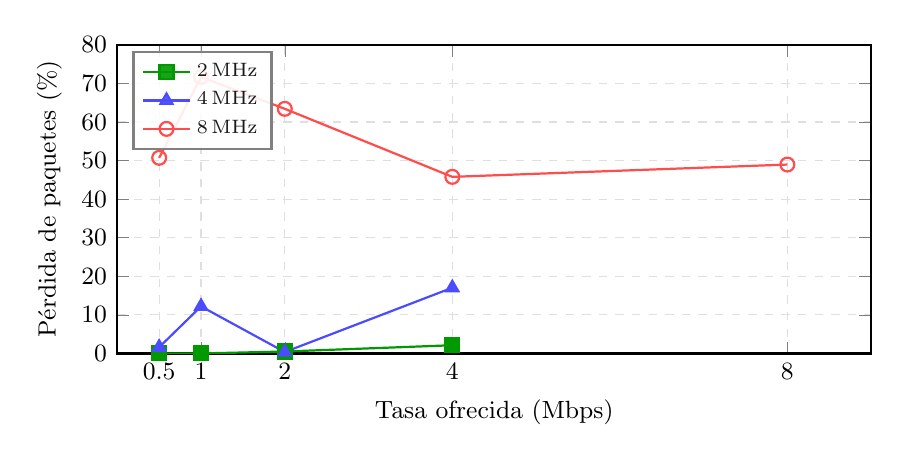
\begin{tikzpicture}
\begin{axis}[
    width=0.92\textwidth,
    height=5.5cm,
    xlabel={Tasa ofrecida (Mbps)},
    ylabel={P\'{e}rdida de paquetes (\%)},
    xmin=0, xmax=9,
    ymin=0, ymax=80,
    xtick={0.5,1,2,4,8},
    ytick={0,10,20,30,40,50,60,70,80},
    grid=major,
    grid style={gray!25, dashed},
    tick label style={font=\small},
    label style={font=\small},
    legend style={at={(0.02,0.98)}, anchor=north west, font=\scriptsize,
                  draw=black!50, fill=white, fill opacity=0.9},
    mark size=2.5pt,
    thick,
]

% 2 MHz
\addplot[color=green!60!black, mark=square*, thick] coordinates {
    (0.5, 0.0) (1, 0.0) (2, 0.50) (4, 2.13)
};

% 4 MHz
\addplot[color=blue!70, mark=triangle*, thick] coordinates {
    (0.5, 1.62) (1, 12.20) (2, 0.37) (4, 17.04)
};

% 8 MHz
\addplot[color=red!70, mark=o, thick] coordinates {
    (0.5, 50.72) (1, 71.69) (2, 63.43) (4, 45.79) (8, 48.98)
};

\legend{2\,MHz, 4\,MHz, 8\,MHz}

\end{axis}
\end{tikzpicture}

\vspace{3mm}
{\small (b) P\'{e}rdida de paquetes UDP por tasa ofrecida}

\caption[An\'{a}lisis UDP por ancho de banda HaLow]{An\'{a}lisis de rendimiento UDP por ancho de banda del canal IEEE~802.11ah.
(a)~Caudal efectivo recibido: 2\,MHz y 4\,MHz saturan cerca de 1\,Mbps, mientras 8\,MHz se limita a $\sim$0{,}25\,Mbps independientemente de la tasa ofrecida.
(b)~P\'{e}rdida de paquetes: 2\,MHz mantiene p\'{e}rdida $<$3\,\% hasta 4\,Mbps;
el canal de 8\,MHz presenta p\'{e}rdida $>$45\,\% incluso a 0{,}5\,Mbps.
Prueba \texttt{iperf3} UDP 10\,s por tasa, enlace Tube AHM $\leftrightarrow$ Pasarela de borde.}
\label{fig:halow-udp-analysis}
\end{figure}
